\documentclass{article}

\usepackage[pdftex]{graphicx}
\graphicspath{{images/}}

\usepackage{hyperref}
\usepackage{url} \urlstyle{sf}

\usepackage{color}
\def\todo#1{{\color{red}TODO\@: #1}}
\def\addref#1{{\color{red}$[$#1$]$}}

\title{Scheduling of Synchronous Data Flow Models onto Scratchpad Memory-Based Embedded Processors \\
        \large Critical Synthesis}

\author{Simon Bihel}

\begin{document}
\maketitle

\section{Introduction}
This is a synthesis of~\cite{che2013scheduling}.

Scratchpad memory has been adopted in many processors to replace traditional caches.
It has to be explicitly managed and compilers need to take that into account.

Synchronous Data Flow graphs are used to model many applications, and the authors decided to focus on stream applications.

The contribution of the paper is a heuristic for a scheduler that finds a solution that minimises the idle time when accessing the main memory.

Section~\ref{context} presents the context and problem formulation.
Section~\ref{tradeoffs} explains the trade-offs that appear when searching for a solution.
Section~\ref{heuristic} details the proposed heuristic.
Section~\ref{extensions} presents additional optimizations. % that focus on data because that's not the main objective
Section~\ref{evaluation} shows the results of experiments done to compare the heuristic to the state-of-the-art.
In Section~\ref{critic} I evoke a few personal opinions on the paper.

\section{Context}
\label{context}
In this section I present the architecture available to us and the applications that we want to schedule.

\subsection{Scratchpad Memory}
The architecture targeted is an embedded processor with no cache but with a Scratchpad Memory (SPM).
It is a memory with small access time that is managed explicitly.
The SPM acts like a small memory with a heap, a stack, global data, etc.
Because it is small, the programmer (or the compiler) has to carefully import the program code and data.

\subsection{Stream Applications}
Stream applications are periodical and each period consists of tasks to process data.
Tasks are called \textit{actors} and constitute a Synchronous Data Flow (SDF).
Actors take as input \textit{tokens} and produce new tokens that they send to other actors.
An example of stream program is given in \figurename~\ref{fig2_1}.

\begin{figure}
\caption{Segment-region code overlay overview}
\centering
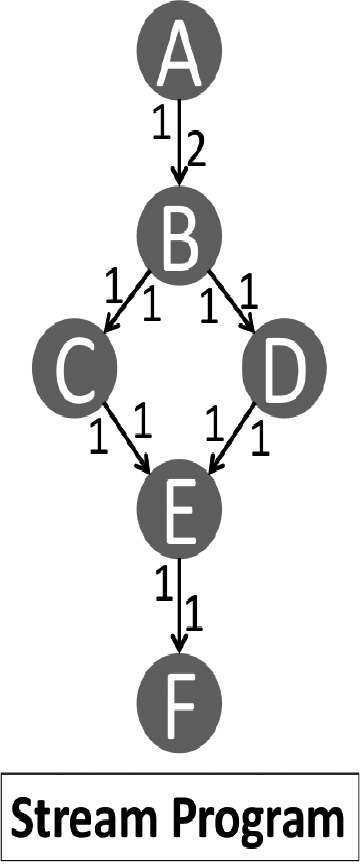
\includegraphics[scale=0.175]{fig2_1}
\label{fig2_1}
\end{figure}

We execute one actor at a time on the processor and the compiler has to produce an order of execution (a Periodical Admissible Sequential Schedule (PASS)) as shown in \figurename~\ref{fig1_2}.

\begin{figure}
\caption{Periodical Admissible Sequential Schedule}
\centering
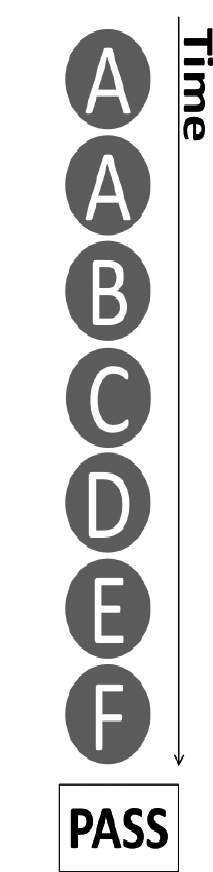
\includegraphics[scale=0.175]{fig1_2}
\label{fig1_2}
\end{figure}

\subsection{Code and Data Overlay}
Because the memory is limited we cannot have all the actors and data at the same time in the SPM\@.
That means that before executing an actor, if it is not already present in the SPM\@, we have to import its code and its data.
To achieve that the authors propose to divide the memory available in \textit{regions}.
Each region in composed on \textit{segments} and only one segment can be present at a time.
Segments are sets of actors (i.e.\ when a segment is in memory, all of its actors are present).
The size of a region is the size of its largest segment which is the sum of its actors code sizes.
Keeping the same example SDF, a possible partition of the SPM is shown in \figurename~\ref{fig2_2}.

\begin{figure}
\caption{Partition of SPM}
\centering
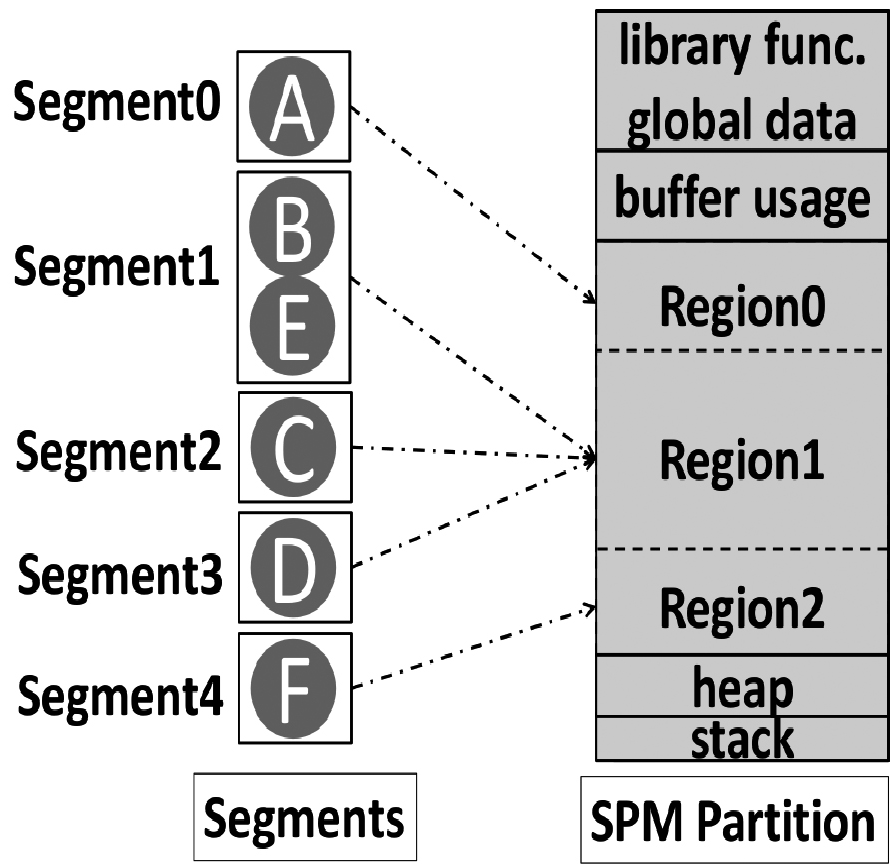
\includegraphics[scale=0.175]{fig2_2}
\label{fig2_2}
\end{figure}

Let's count the number of Direct Access Memory (DMA) transfers, with segments 0, 1 and 4 already loaded at the beginning.
We execute two times A, and then B.
Then we have to load C so we load segment 2 and remove (i.e.\ overlay) segment 1.
Then the same happens for D and segment 3.
Again we have to overlay region 1 and load again segment 1 to execute E.
Finally we can execute F that is already in region 2.
We want to finish in the same state as we start the PASS, and it is already the case in this example.
For one PASS we have made 3 DMA transfers for code overlay purpose.

To avoid waiting for DMA transfers we can \textit{prefetch}.
If we are executing an actor from a certain region, and we know we will have to load an actor for a different region then we can do the transfer during the execution.
An example with a different PASS than previous examples is given in \figurename~\ref{fig3}.
A deep prefetching is simply a prefetch that is done as early as possible, i.e.\ after the last execution of an actor of the same region.

\begin{figure}
\caption{Code prefetching}
\centering
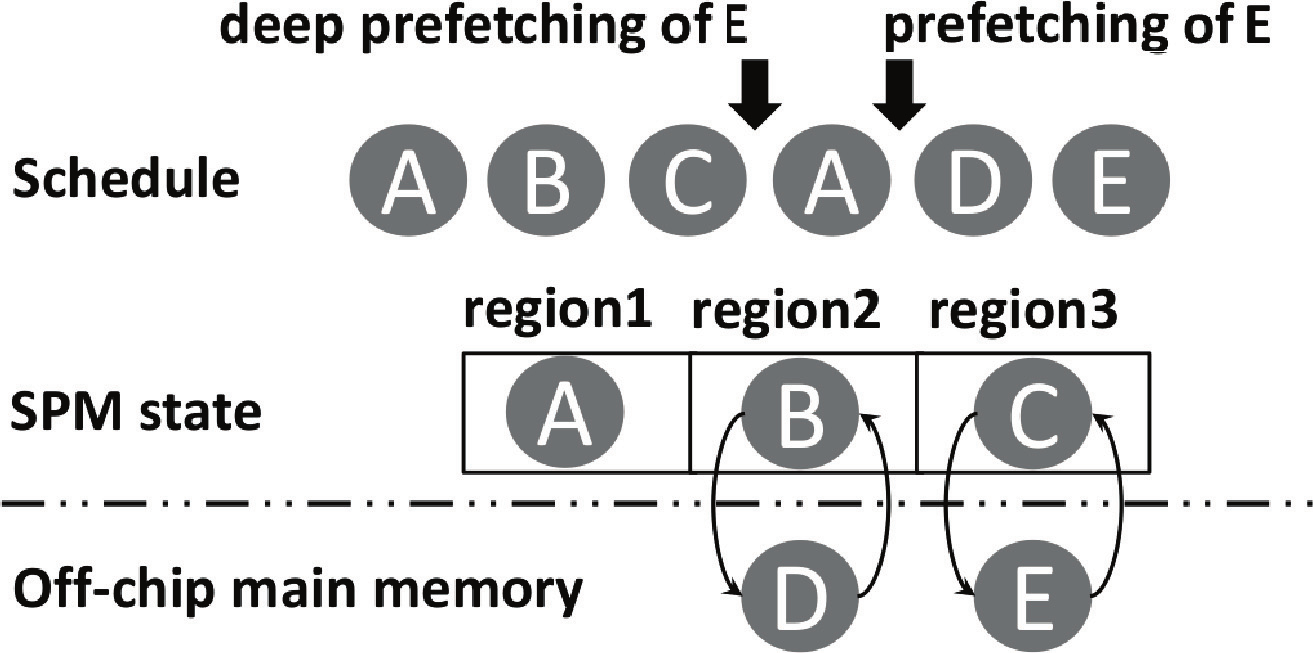
\includegraphics[scale=0.175]{fig3}
\label{fig3}
\end{figure}

The overlay can be used for data also.
If we generate a token that will only be consumed in a long time, we can put it in the main memory and fetch it again when necessary.
This way, some memory in the SPM is freed, the \textit{buffer usage} (i.e. SPM part for data) is reduced, which can allow to have more regions and thus reduce the number of code overlay for example.

A limitation of the prefetching is that the DMA engine can only do a transfer at a time.
Because of that we cannot do all the prefetch optimizations that we would like.

% \begin{figure}
% \caption{DMA engine usage}
% \centering
% 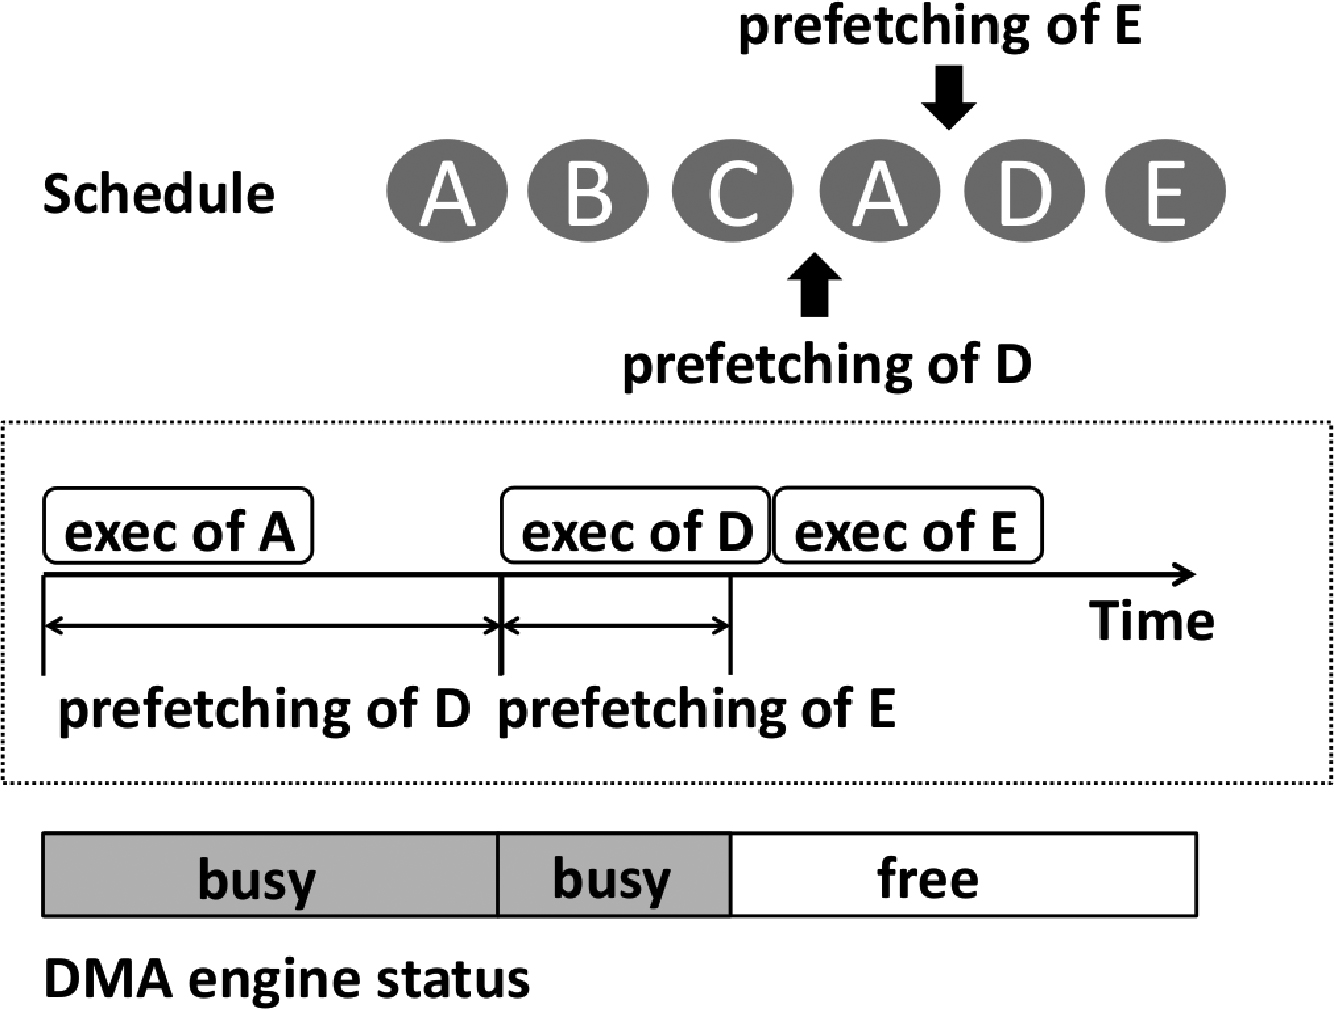
\includegraphics[scale=0.175]{fig4}
% \label{fig4}
% \end{figure}


\section{Trade-offs}
\label{tradeoffs}
In this section I present the characteristics of a PASS and how we evaluate its efficiency.

\subsection{PASS Generation}
To design the heuristic, the authors propose to focus on two properties of the scheduling.
\begin{description}
  \item[Buffer Usage] a reduced total memory required for storing data means that the partition for the code can be larger.
  \item[Actor Switches] grouping the executions of the same actor will probably reduce the number of code overlay.
\end{description}

We need to take these two criteria into account.
Firstly, we need to keep the buffer usage below a certain threshold or there will not be enough space for the code.
Secondly, neither a Minimum Buffer Schedule or a Minimum Switch Schedule will always be optimal for our code overlay minimization problem.

\subsection{Actor to Region Assignment and Segmentation}
Having actors that are executed one after another in the same segment can reduce the code overlay overhead.
But maybe the segment would be too big so you might want to have them in separate regions to allow prefetching and avoid evicting them consecutively.
Having large segments will also result in larger DMA transfers.

\subsection{Data Overlay}
Data overlay brings more stress on the DMA engine so using it can decrease of the buffer usage at the expense of data overlay overhead (i.e.\ idle time).

\section{SDF Scheduling Heuristic}
\label{heuristic}
This section presents the basic heuristic to schedule an SDF while minimizing the code overlay overhead.

The basic heuristic does not take into account prefetching nor data overlay.
This simplification makes to calculation of the code overlay overhead easier.
The PASS is executed symbolically, keeping track of the memory state, and when we need to transfer a segment the code overlay counter is increased according to the size of the segment.

For the region assignment, the algorithm start by placing each actor in its own region.
And iteratively, while the regions are using more memory than available, two region are collapsed in a single region.
The choice is made on regions that have actors that interact the least between them.
That way we avoid doing code overlay over and over again for the same region.
This is a greedy algorithm and no segmentation is used.

For the segmentation we start with actors from the same region, and each actors is in its own segment.
In greedy manner, segments are collapsed as long as the new segment does not go over the region size and as long as the code overlay improves.

The main algorithm for the scheduler is in \figurename~\ref{algo2}.
We start with a Minimum Buffer Schedule using the algorithm of~\cite{jantsch2004modeling} and evolve towards a Minimum Switch Schedule.
The goal is to group same actors in the PASS (we judge if a new PASS is legal by checking that the numbers of tokens exchanged are not negative).
% TODO

Region assignment and segmentation are both in $O(n^3)$ and it is done for each loop of PASS generation, which is in $O(n)$.
The overall complexity of the heuristic is $O(n^4)$.

\begin{figure*}
\caption{Basic heuristic}
\centering
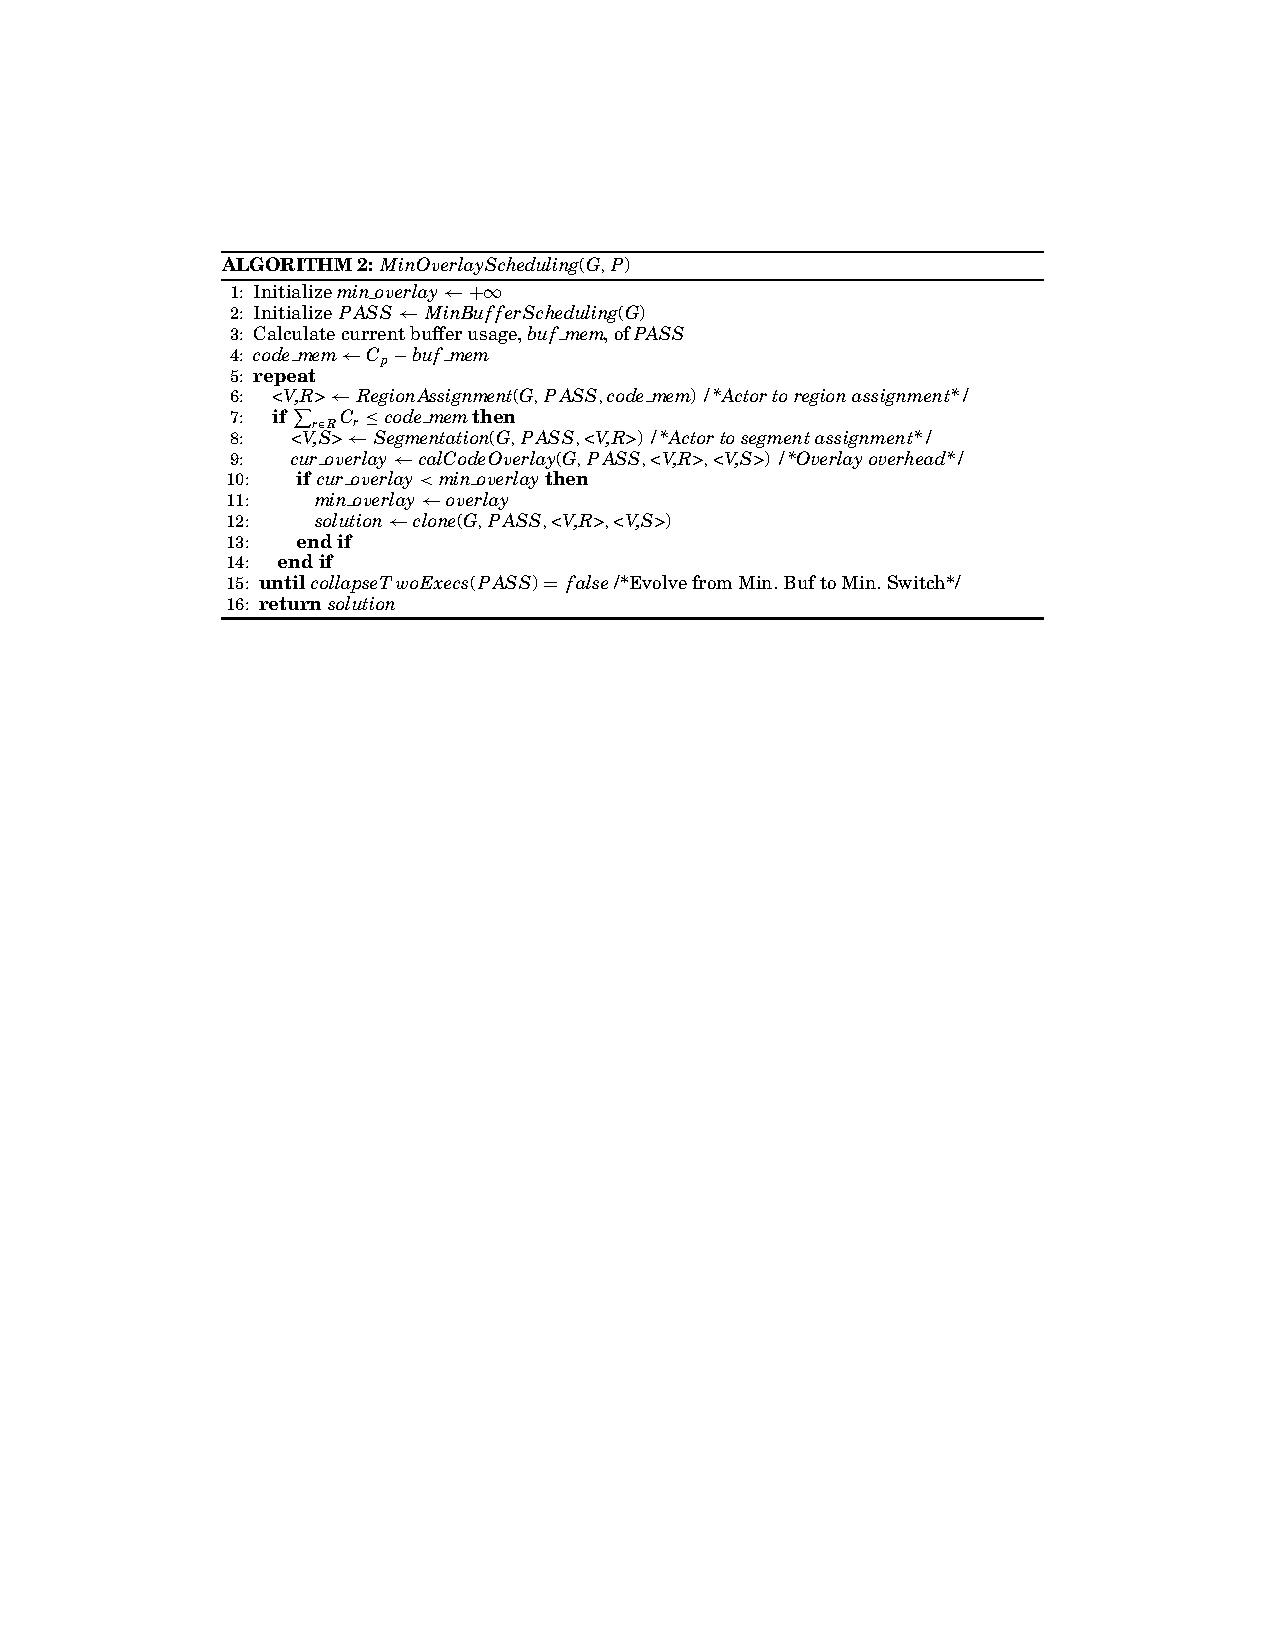
\includegraphics[scale=0.92]{algo2}
\label{algo2}
\end{figure*}


\section{Extensions}
\label{extensions}
This section presents the integration of prefetching and data optimizations.

\subsection{Prefetching}
Adding prefetching changes only the function to calculate the code overlay.
In addition to keeping track of the memory state, we also have to keep track of the DMA engine's usage.
When executing the PASS we need to look forward to see if we need to start a transfer before firing the current actor.
The complexity does not change because we always see 1 step ahead in the case of basic prefetching, and for deep prefetching we look on average a constant ahead.

\subsection{Data Overlay}
To integrate data overlay, we need to change the way we assign region.
To keep track of the varying size of the data buffer, alike the code overlay calculation, we need to execute the PASS\@.
% TODO

\section{Evaluation}
\label{evaluation}
Extensive experiments were conducted.
The authors compared their heuristic to state-of-the-art scheduler.
Then the impact of each optimization has been studied.
Comparison between Minimum Buffer Schedule and Minimum Switch Schedule has been done.
Finally, experiments for different architecture characteristics were conducted.

They used a set of stream SDF benchmarks.

\subsection{State-of-the-art Comparison}
The state-of-the-art is a 3-stage Integer Linear Program with Minimum Buffer Scheduling as target.
They compare to this ILP (basic and MBS target), to the basic MBS, and 4 variants of their heuristic with or without optimizations.

They always do better when the absence of code overlay cannot be achieved easily.

\subsection{Optimizations Impact}
Prefetching delivers an average performance gain of 17\% but deep-prefetching and data overlay are almost insignificant.
This is due to the limitation of the DMA engine.

\subsection{Heuristic Focus Comparison}
Evolving toward a Minimum Switch Schedule generally reduces the overhead increasingly.

\subsection{Architecture Scaling}
Increasing the SPM size generally results in better results but not always due to the greedy nature of the segmentation algorithm.

Increasing the DMA cost increasing much faster the overlay overhead and reduce the impact of deep-prefetching and data overlay.

Increasing the code size makes it often impossible to find a solution with all optimizations.


\section{Conclusion}
\label{critic}
The proposed heuristic stays reasonable in complexity but still gives better results than existing solutions for non trivial problems.


\bibliographystyle{alpha}
\bibliography{biblio}

\end{document}
